\chapter{Usage}\label{Usage}
This chapter will describe the systems interaction with its surroundings. This will be done by making an actor specification and then presenting a user pattern diagram, which will be showcased in an state machine.

\section{Actor specification}
\label{Actor_specification}
An actor will be described by a actor specification , the actor is a user of the system.

\hrule
\begin{tightcenter}
\textit{\textbf{User}}
\end{tightcenter}
\hrule
\textbf{Objective:} A person who prepare their meals them self, either for them self or for a family household. The user's primary need is to plan their their week in order to efficiently shop their groceries and lessen food waste.\\

\textbf{characteristic:} The system includes a user base of which the users have different needs and preferences.

\textbf{Examples:} User A is an allergic and has to make meals which excludes nuts. When A is shopping she needs to look at the package info to make sure that the product does not contain trace of nuts.

User B is a young student who is in a relationship. User B has a tight budget and a little time frame to shop in. B finds it difficult to sustain an overview of their share storage of food. Therefore B will sometimes buy products they do not need, for example, B might purchase milk even though they already have three litres stored. This will sometime result in them not being able to use all the milk before it expires, which is bad for their shared budget and food waste.
\hrule



\section{User pattern}
The user pattern shows an abstraction between the interactions i the system and actor. To show these interactions an state machine diagram have been chosen. The diagram shows the how the dynamic states can shift trough interactions with the actor. Even tough many of the details is excluded, it still gives a good overview of how the logic i set up in the user pattern and how the the dynamic flow goes. 

The purpose of the diagram is to create an overview of the application domains interactions with the system. This will be used to find acquirements for the functions and user interface. There are three user pattern diagrams, each representing different areas of the system. The three diagrams showcase the user patterns in the:
\begin{itemize}
\item{Shopping list}
\item{Foodplan}
\item{Inventory}
\end{itemize}

When the user actor traverses trough the system, the actor will undertake one of two roles. An administrative or a planning oriented role.
The first diagram is the one for the Shopping list, in this part of the system the user actor operates under the administrative role.
The option to go back or cancel have not been drawn on the diagrams as there only contribution is to make the diagrams less readable and add redundant repetitions, that goes for all of the diagrams.

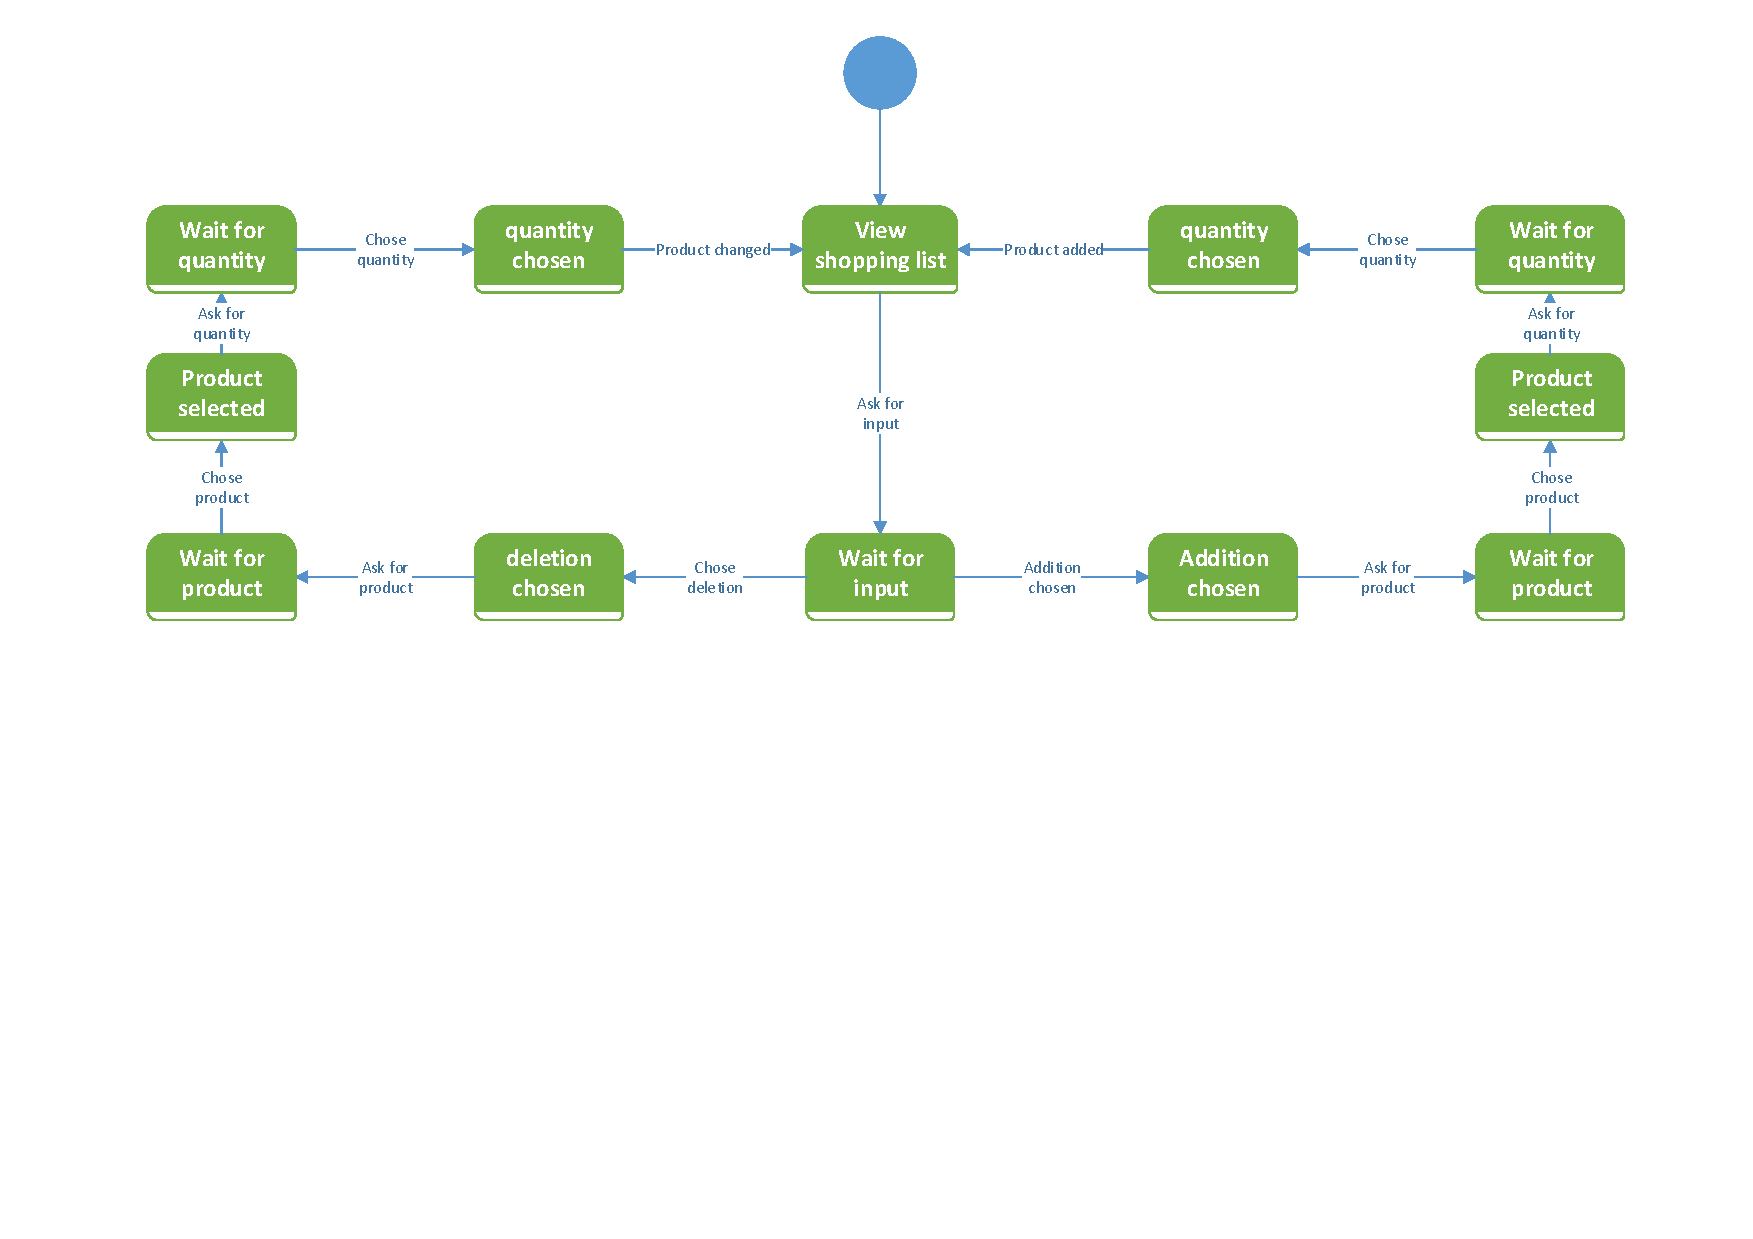
\includegraphics[width=1.0\textwidth]{ApplicationDomain/upShoppingList.pdf} \label{Shopping_List_Figure}
When the user goes to the shopping list, the program will wait for him to either add or delete an product. If he chooses to add ana product to the list, he will be asked to chose a product. The product also needs a quantity that specifies how much of the product is needed to be listed (2 litres of milk or ½ kilo of flour). If an valid quantity is given it will be added to the shopping list an the user will be able to add or delete another product. The only quantity that is not acceptable is value that is below or equal to zero.

The user is also able to delete a product from the shopping list. The user will then have to chose an item already present on the list and then chose how much of the product tat should be removed from the list. If the user chooses a quantity that will leave the product at a zero quantity the product will be removed altogether from the list. For example if the list contains four apples, and the user removes three apples, one apple will still be present on list. However, if the user decided to remove four apples, the list will no longer contain the product apples. It should be noted that trying to remove a quantity of a product that will leave i a negative value will result in an error.


The second diagram is the one for the foodplan, in this part of the system the user actor operates under the planing role.

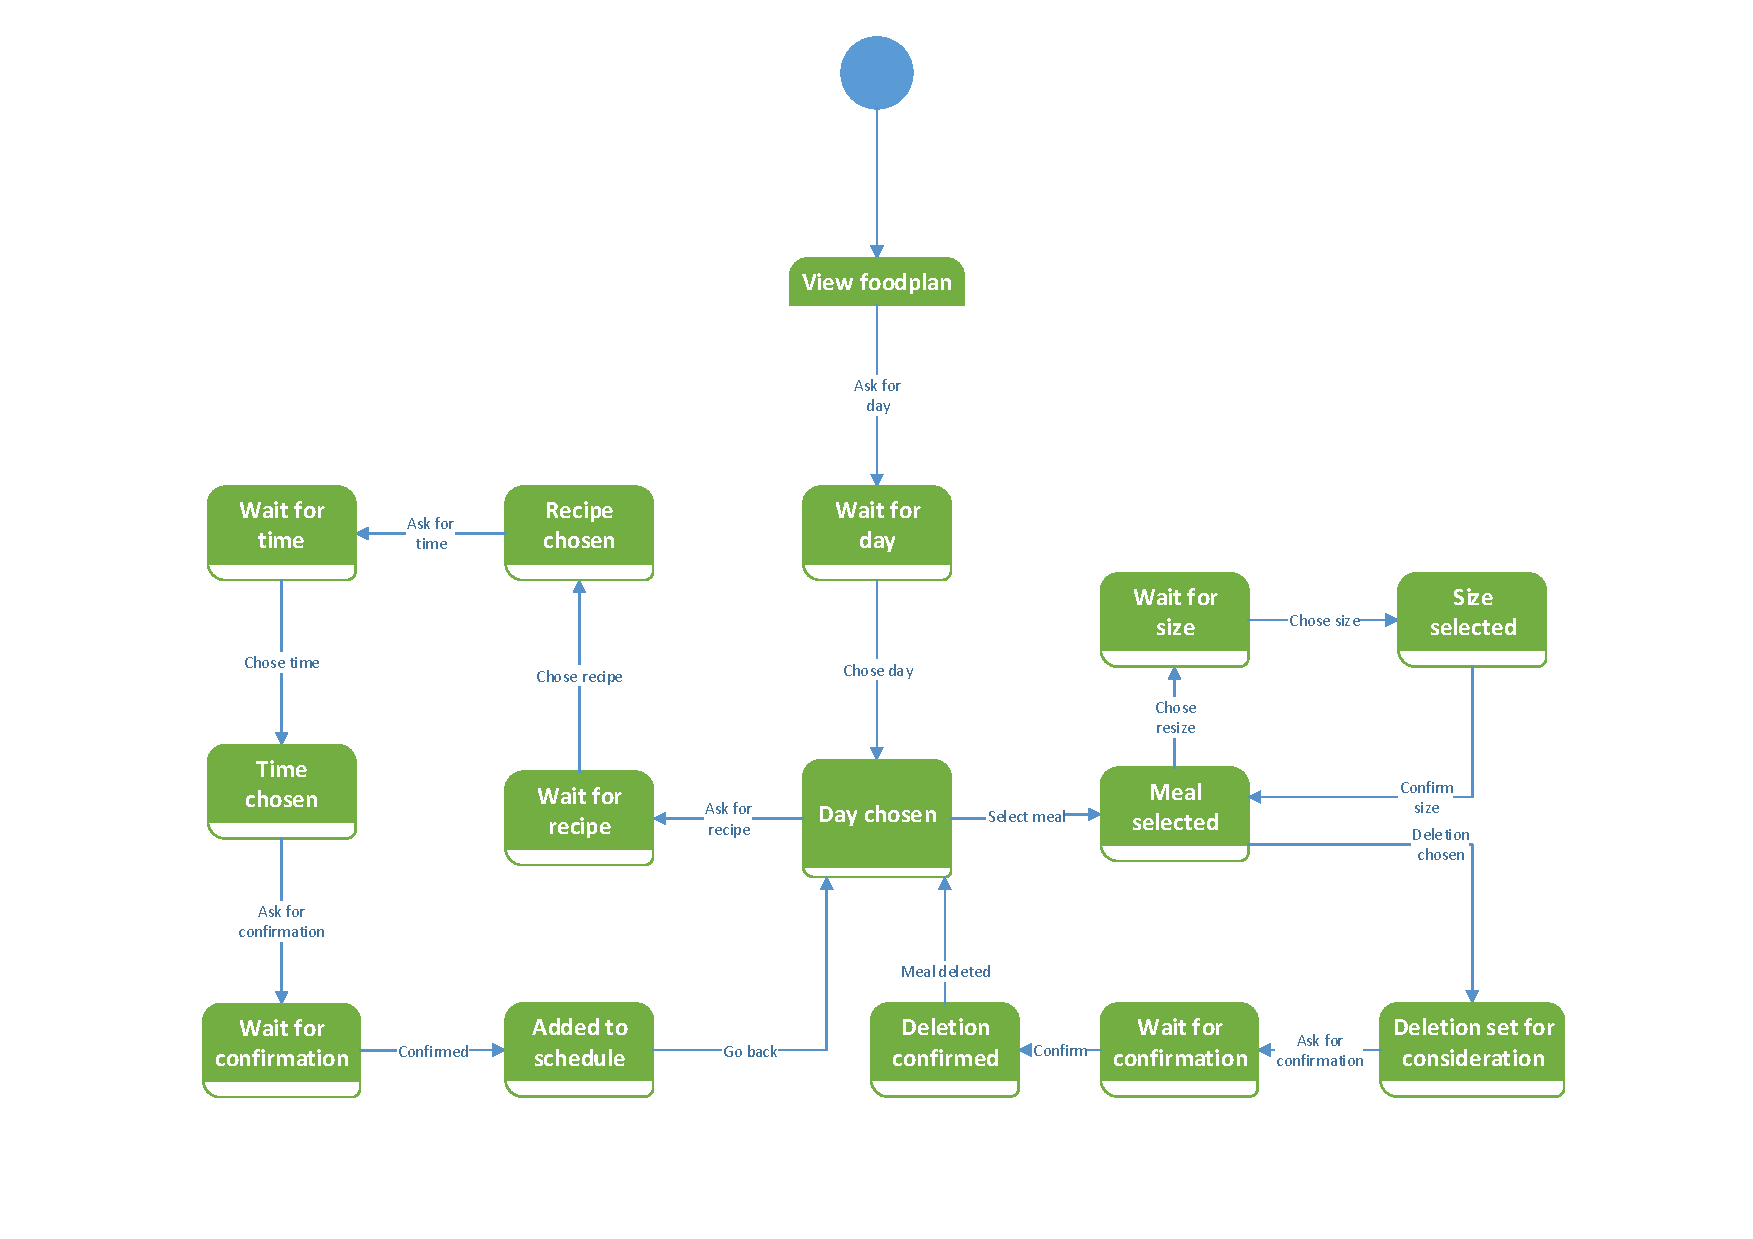
\includegraphics[width=1.0\textwidth]{ApplicationDomain/spViewFoodPlan.pdf} \label{Foodplan_Figure}

\newpage